      
               
                \begin{ledgroupsized}[r]{120mm}
                \footnotesize 
                \pstart                
                \noindent\textbf{\"{U}berlieferung:}   
                \pend
                \end{ledgroupsized}
            
              
                            \begin{ledgroupsized}[r]{114mm}
                            \footnotesize 
                            \pstart \parindent -6mm
                            \makebox[6mm][l]{\textit{L}}Konzept: LH XXXV 5, 2 Bl. 7\textendash8. 1 Bog. 2\textsuperscript{o}. 4 S. Bl. 9, 20 x 17 cm. Mit Ausnahme des linken Randes von Blatt 9 alle anderen R\"{a}nder beschnitten, der untere Rand schr\"{a}g. R\"{u}ckseiten von Bl. 8 und Bl. 9 leer. Auf Bl. 7~v\textsuperscript{o} in der linken oberen Ecke eine Zeichnung, die im Druck nicht wiedergegeben wird, da es sich um eine erste fl\"{u}chtige Skizze von \textit{[Fig. 7]} handelt. Die drei Zeichnungen von Bl. 9 am linken Rand verteilt, Text umlaufend. Datierungen und Titel wurden sp\"{a}ter hin\-zugef\"{u}gt. Wie N. 53 ist auch dieses St\"{u}ck im Zusammenhang mit \cite{00261}\textit{LSB} VII, 3 N. 39 sowie LH XXXV 5, 2 Bl. 1 zu sehen.\\Cc 2, Nr. 825, 826
                            \pend
                            \end{ledgroupsized}
              
                            \begin{ledgroupsized}[r]{114mm}
                            \footnotesize 
                            \pstart \parindent -6mm
                            \makebox[6mm][l]{\textit{E}}\textsc{H.-J. Hess}, \cite{00188}\textit{Die unver\"{o}ffentlichten naturwissenschaftlichen und technischen Arbeiten von G. W. Leibniz aus der Zeit seines Parisaufenthaltes. Eine Kurzcharakteristik}, in: \textit{Leibniz \`{a} Paris}, Bd. 1, Wiesbaden 1978 (= \textit{Studia Leibnitiana}, Suppl. XVII), darin S.~211\textendash217 (Teildruck). 
                            \pend
                            \end{ledgroupsized}
                %\normalsize
                \vspace*{5mm}
                \begin{ledgroup}
                \footnotesize 
                \pstart
            \noindent\footnotesize{\textbf{Datierungsgr\"{u}nde}: Auf Bl. 7 r\textsuperscript{o} und 9 r\textsuperscript{o} von Leibniz datiert.}
                \pend
                \end{ledgroup}
            
                \vspace*{8mm}
                    \pstart
  \centering          \lbrack\textit{Teil 1}\rbrack
            \pend
                \pstart 
                \normalsize\selectlanguage{latin}
            [7 r\textsuperscript{o}] Decembris 1674.
            \pend 
            \pstart\normalsize   \begin{center}\textso{Calculus Elasticus}\\\textso{ubi et quomodo alia problemata methodi tang. inversae reducantur subinde ad quadraturas.}\footnote{\textit{In der rechten oberen Ecke}: Vid. sub \textso{finem.}}\end{center}\edtext{}{\lemma{\textso{Calculus}}\linenum{|18|||20|}\Afootnote{\textit{bis} \textso{quadraturas.} \textit{doppelt unterstrichen}}}\edtext{}{\lemma{\textso{finem}}\linenum{|21|||21|}\Afootnote{\textit{doppelt unter\-strichen}}}%\footnote{\textit{In der rechten oberen Ecke}: Vid. sub \textso{finem.}}
            \pend
            \clearpage
%  Zeitz auskommentiert                  \begin{center}
%             % \begin{wrapfigure}{l}{0.4\textwidth}         
%             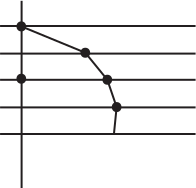
\includegraphics[width=0.2\textwidth]{images/35_5_7r2}           
%                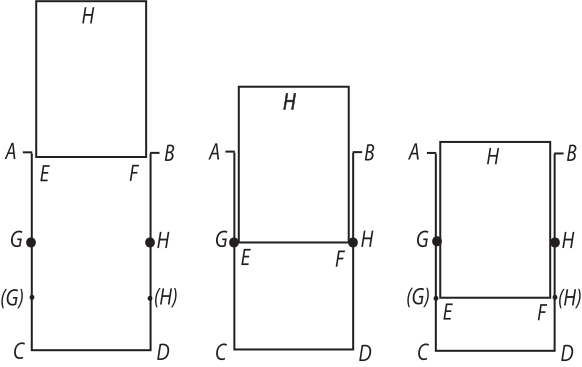
\includegraphics[width=0.7\textwidth]{images/35_5_7r1}\\\textit{[Fig. 1]}\hspace{1.5cm}\textit{[Fig. 2]}\hspace{2cm}\textit{[Fig. 3]}\hspace{2cm}\textit{[Fig. 4]}\\
%                        %\caption{Bildbeschreibung}
%                        %\end{wrapfigure}
%                        %@ @ @ Dies ist eine Abstandszeile - fuer den Fall, dass mehrere figures hintereinander kommen, ohne dass dazwischen laengerer Text steht. Dies kann zu einer Fahlermeldung fuehren. @ @ @ \\
%                     % \begin{wrapfigure}{l}{0.4\textwidth}                    
%           %     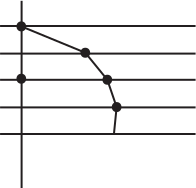
\includegraphics[width=0.2\textwidth]{images/35_5_7r2}\\\textit{[Fig. 1]}
%                        %\caption{Bildbeschreibung}
%                        %\end{wrapfigure}
%                        %@ @ @ Dies ist eine Abstandszeile - fuer den Fall, dass mehrere figures hintereinander kommen, ohne dass dazwischen laengerer Text steht. Dies kann zu einer Fahlermeldung fuehren. @ @ @ \\
%                        \end{center}
                  \pstart   Sit \textit{ABCD} cylinder \edtext{cavus}{\lemma{}\Afootnote{cavus \textit{ erg.} \textit{ L}}} aere plenus a parte \textit{CD} clausus, a parte \textit{AB} apertus. Huic perfecte \edtext{in \textit{EF}}{\lemma{}\Afootnote{in \textit{EF} \textit{ erg.} \textit{ L}}} congruat embolus\protect\index{Sachverzeichnis}{embolus} \edtext{seu cylinder convexus \textit{HEF}}{\lemma{embolus}\Afootnote{ \textit{ (1) }\ \textit{HEF}, \textit{ (2) }\ seu cylinder convexus \textit{HEF} \textit{ L}}} et ponatur cylinder convexus intrudi in concavum, usque ad \textit{GH} \edtext{vel \textit{(G)(H)}}{\lemma{}\Afootnote{vel \textit{(G)(H)} \textit{ erg.} \textit{ L}}}, necesse est aerem ea \edtext{intrusione}{\lemma{ea}\Afootnote{ \textit{ (1) }\ compressione\protect\index{Sachverzeichnis}{compressio|textit} \textit{ (2) }\ intrusione \textit{ L}}} comprimi. Ponatur aeris in vase contenti \edtext{portiuncula}{\lemma{contenti}\Afootnote{ \textit{ (1) }\ quantitas esse \textit{ (2) }\ minimum aliquod co \textit{ (3) }\ spatium aliquo \textit{ (4) }\ portiuncula \textit{ L}}} quadam minor quam quae \edtext{possit assignari}{\lemma{quae}\Afootnote{ \textit{ (1) }\ assumi \textit{ (2) }\ possit assignari \textit{ L}}}, esse $\beta$. Numerus ipsarum  $\beta$ quas capiat recta \textit{AB} $\sqcap$ \textit{c} ponatur esse \textit{c$\beta$} et recta \textit{BD} ponatur esse \textit{d}, erit \edtext{quantitas aeris}{\lemma{erit}\Afootnote{ \textit{ (1) }\ quantitas nu \textit{ (2) }\ quantitas aeris \textit{ L}}} \textit{cd$\beta$}. Quantitas autem spatii \textit{cd$\gamma$}. Sumta \edtext{infinite parva $\gamma$. Ponatur jam et \textit{AG}}{\lemma{Sumta}\Afootnote{ \textit{ (1) }\ recta \textit{AG} \textit{ (2) }\ infinite [...] \textit{AG} \textit{ L}}} esse infinite parva $\sqcap$ $\gamma$ et aerem omnem \textit{cd$\beta$}, intrudi in spatium $cd-c\gamma$ seu usque ad \textit{GH} vel \edtext{etiam}{\lemma{vel}\Afootnote{ \textit{ (1) }\ item \textit{ (2) }\ etiam \textit{ L}}} ponatur aerem omnem intrudi usque ad \textit{(G)(H)}, ponendo \textit{A(G)} $\sqcap$ 2$\gamma$ erit aer intrusus in spatium $cd-2c\gamma$ et erit vis aeris\protect\index{Sachverzeichnis}{vis!aeris compressi} restitutionem molientis ex \textit{GH}, ad vim aeris\protect\index{Sachverzeichnis}{vis!aeris compressi} restitutionem molientis ex \textit{(G)(H)}, \edtext{ut}{\lemma{\textit{(G)(H)},}\Afootnote{ \textit{ (1) }\ ut \textit{ (2) }\ in \textit{ (3) }\ ut \textit{ L}}} \edtext{quantitates mutationum}{\lemma{ut}\Afootnote{ \textit{ (1) }\ gradus compressionum. \textit{ (2) }\ quantitates mutationum \textit{ L}}} a statu naturali\protect\index{Sachverzeichnis}{status naturalis} \edtext{deflectentium}{\lemma{naturali}\Afootnote{ \textit{ (1) }\ . Nempe \textit{ (2) }\ deflectentium \textit{ L}}}. Nimirum considerandum est in prima compressione\protect\index{Sachverzeichnis}{compressio} effectum esse, ut totus aer quia implebat \textit{cd} impleat tantum $cd-c\gamma$. Ergo quodlibet aeris minimum $\beta$ est in spatio quod sit ad spatium $\gamma$ sibi naturaliter debitum, ut $cd-c\gamma$ est ad \textit{cd} eritque proinde spatium quod nunc implet $\sqcap\hspace{5.5pt} cd\gamma-c\gamma^2\smallsmile cd\sqcap d\gamma-\gamma^2, \smallsmile d$. Quod si pro $\gamma$ ponamus 2$\gamma$, \edtext{vel}{\lemma{2$\gamma$,}\Afootnote{ \textit{ (1) }\ ut \textit{ (2) }\ vel \textit{ L}}} etiam 3$\gamma$, etc., vel generaliter \textit{y}, \edtext{tunc spatium}{\lemma{\textit{y},}\Afootnote{ \textit{ (1) }\ fiet \textit{ (2) }\ tunc spatium \textit{ L}}} quod implet ipsum $\beta$ minimum aeris erit: $dy-y^2\smallsmile d$. \edtext{Jam}{\lemma{$dy-y^2\smallsmile d$.}\Afootnote{ \textit{ (1) }\ Sunt autem vires seu conatus\protect\index{Sachverzeichnis}{conatus|textit} ad restituendum, in quolibet puncto aeris,  \textit{(a)}\ ut \textit{(b)}\ in ratione compressionum\protect\index{Sachverzeichnis}{compressio|textit} seu differentiarum a statu naturali\protect\index{Sachverzeichnis}{status naturalis|textit}; \textit{ (2) }\ Jam \textit{ L}}} aestimandum est, qua ratione recte possint aestimari vires seu conatus\protect\index{Sachverzeichnis}{conatus} ad restitutionem; \edtext{an scilicet sint ut differentiae}{\lemma{restitutionem;}\Afootnote{ \textit{ (1) }\ an a differenti \textit{ (2) }\ an scilicet sint ut differentiae \textit{ L}}} spatiorum quae implent; ac proinde vis aeris compressi\protect\index{Sachverzeichnis}{vis!aeris compressi} usque ad \textit{AG}, foret ad vim aeris compressi\protect\index{Sachverzeichnis}{vis!aeris compressi} usque ad \textit{A(G)} ut est \textit{AG} ad \textit{A(G)}. Sed hoc absurdum esse demonstratur, quia ita 
%  Zeitz auskommentiert                   \begin{wrapfigure}{l}{0.3\textwidth}                    
%                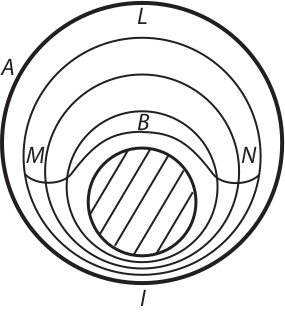
\includegraphics[width=0.3\textwidth]{images/35_5_7r3}\\\rule[0cm]{1.5cm}{0cm}\textit{[Fig. 5]}
%                        %\caption{Bildbeschreibung}
%                        \end{wrapfigure}
%                        %@ @ @ Dies ist eine Abstandszeile - fuer den Fall, dass mehrere figures hintereinander kommen, ohne dass dazwischen laengerer Text steht. Dies kann zu einer Fahlermeldung fuehren. @ @ @ \\
                        comprimi posset aer ad minimum usque spatium; quod est impossibile; itaque sic potius statuendum est esse vires in reciproca spatiorum ratione. Quod ut appareat considerandum est: vim\protect\index{Sachverzeichnis}{vis!elastica} omnem Elasticam non oriri a defectu spatii debiti; nullum enim spatium debitum est Elasticis, sed si possent \edtext{amplius semper atque amplius}{\lemma{possent}\Afootnote{ \textit{ (1) }\ altius semper atque altius \textit{ (2) }\ amplius semper atque amplius \textit{ L}}} aperirentur; verum parvitas spatii eruntque \edtext{adeo virium magnitudines, ut}{\lemma{adeo}\Afootnote{ \textit{ (1) }\ vires ut \textit{ (2) }\ virium magnitudines, ut \textit{ L}}} spatiorum parvitates. Sive erunt virium magnitudines in magnitudinis 
                  spatiorum reciproca ratione. Quod et physicis rationibus ostendi posset; \edtext{dubitandum enim non videtur vim Elaterii oriri a motus celeritate in iis quae sunt compressa}{\lemma{posset;}\Afootnote{ \textit{ (1) }\ erunt enim vires ut celeritates\protect\index{Sachverzeichnis}{celeritas|textit} \textit{ (2) }\ dubitandum [...] compressa \textit{ L}}},  ut in vacuo vase aqua pleno \edtext{\textit{A}}{\lemma{}\Afootnote{\textit{A} \textit{ erg.} \textit{ L}}} ponatur aqua vi quadam concitata moveri 
                                    (ut si vas circa suum centrum agatur motu aequabili\protect\index{Sachverzeichnis}{motus!aequabilis} et durante) in aqua fluctuare intelligatur globus quidam \textit{B}, eccentrice positus, ille motum reddet inaequabilem, fiet enim, ut motus sit celerior in \textit{I}, quam in \textit{L}, quia eodem tempore tantundem transit spatii per \textit{I}, quantum per \textit{L}, et \edtext{quia celeritas oritur ab intrusione, ideo non est dubitandum celeritatem}{\lemma{et}\Afootnote{ \textit{ (1) }\ ideo celeritas\protect\index{Sachverzeichnis}{ celeritas|textit} \textit{ (2) }\ quia [...] celeritatem \textit{ L}}} illam conari rejicere globum in aquae medium. Considerandum autem causam istam esse a materiae consistentia, et ex principio, \edtext{quod fortiter mota}{\lemma{quod}\Afootnote{ \textit{ (1) }\ motus \textit{ (2) }\ fortiter mota \textit{ L}}} rejiciunt a se quae ipsa contingunt cujus rei ratio est, quod quae moventur, agunt in omnes partes, quomodocunque moveantur. Notandum autem alios atque alios esse gradus velocitatum\protect\index{Sachverzeichnis}{gradus celeritatis} quia aliae atque aliae 